\documentclass{article}
\usepackage{caisc_2026}
\usepackage[utf8]{inputenc}
\usepackage[T1]{fontenc}
\usepackage{hyperref}
\usepackage{url}
\usepackage{booktabs}
\usepackage{amsfonts}
\usepackage{amsmath}
\usepackage{nicefrac}
\usepackage{microtype}
\usepackage{xcolor}
\usepackage{graphicx}
\usepackage{multirow}

\hypersetup{
  colorlinks=true,
  linkcolor=blue,
  citecolor=blue,
  urlcolor=blue
}

\title{A Polarity Axis, Not a Logical Operator:\\
Linear Structure of Negation in a Reasoning LLM}

\author{Anonymous Author(s) \\ Anonymous Institution \\ \texttt{[anonymous for review]}}

\begin{document}

\maketitle

\begin{abstract}
The Linear Representation Hypothesis (LRH) proposes that concepts are encoded as linear directions in language model residual streams.
We ask whether this extends to \emph{logical operators}: does a model learn a single universal direction $\mathbf{d}_{\neg}$ that implements negation across semantic content?
Using DeepSeek-R1-Distill-Qwen-7B, we construct a multi-morphology paired dataset spanning six syntactic negation forms (\textit{not}, \textit{n't}, \textit{never}, \textit{no X}, \textit{fails to}, \textit{it is false that}) and a held-out antonym test set (no \textit{not} token).
We apply SVD to residual-stream activation deltas across all pairs and find a near-degenerate one-dimensional structure emerging sharply at layer 4 (top-1 explained variance 0.986), persisting through layer 20.
The extracted direction $\mathbf{d}_{\neg}$ is collinear with the antonym-pair direction ($|\cos| = 0.998$), even though antonym pairs contain no surface negation token---consistent with a direction that generalises beyond the \textit{not} token.
However, the non-logical-\textit{not} control (``not only\ldots but also'') is \emph{also} collinear with $\mathbf{d}_{\neg}$ ($|\cos| = 0.999$) and shows comparable perturbation transfer, so we cannot cleanly separate a \emph{logical} negation direction from a more general \textit{not}/polarity direction; we report this rather than claim a clean logical-vs-lexical dissociation.
We also note that with only 8 antonym test pairs these estimates carry substantial variance.
We test the operator hypothesis directly with a \textbf{double-negation experiment}: if $\mathbf{d}_{\neg}$ implements a logical operator, applying it twice (at $\alpha = +2$) should partially cancel the first application (returning toward the unsteered distribution), whereas a polarity feature would push monotonically further.
Steering at layer~5 across 8 factual prompts produces logit distributions with mean cosine to baseline $\approx 1.000$ at all $\alpha \in \{+1, +2, +3, -1, -2\}$---no measurable behavioral change at any scale.
This null result is consistent with $\mathbf{d}_{\neg}$ being a correlational artifact rather than a causally relevant direction, and confirms the polarity-axis rather than operator interpretation.
All six training morphologies, including quantifier negation (``No X is Y''), collapse onto a single one-dimensional axis ($|\cos|\approx 0.99$); because SVD singular-vector signs are arbitrary, we do \emph{not} interpret this as predicate and quantifier negation occupying ``opposite poles.''
A perturbation experiment shows that adding $\alpha \cdot \hat{\mathbf{d}}_{\neg}$ (the unit direction, at a norm-matched scale with $\alpha$ in units of the mean layer-5 residual norm) produces logit shifts that increase monotonically with $|\alpha|$ and exceed a random-direction baseline at large $|\alpha|$ ($\approx 2\times$ at $|\alpha|=2$).
\end{abstract}

%% -----------------------------------------------------------------------
\section{Introduction}
\label{sec:intro}

A key property attributed to modern language models is that high-level concepts are represented as linear directions in the residual stream~\citep{park2024linear}.
This view, called the \emph{Linear Representation Hypothesis} (LRH), has motivated a range of techniques for model steering~\citep{zou2023representation} and circuit analysis.
Much of the supporting evidence concerns \emph{object-level concepts} such as factual attributes or emotional states.
Whether LRH extends to \emph{logical operators}---transformations that systematically relate concepts to their semantic complements---is an open question with both scientific and safety implications.

Negation is the simplest logical operator: ``it is hot'' becomes ``it is not hot''; ``happy'' becomes ``unhappy'' via antonymy.
If a single linear direction $\mathbf{d}_{\neg}$ implements logical negation universally across semantic content, then:
(a) adding $\mathbf{d}_{\neg}$ to any concept's representation should flip it to its negation, and
(b) the direction should be learnable from one syntactic form and transfer to others, including forms with no surface ``not'' token.

The alternative hypothesis is that ``negation'' is merely an artifact of the word \textit{not}: the model learns a direction for the \textit{not} token, not for the abstract logical operation.
We design our experiments to distinguish these two hypotheses.

We use DeepSeek-R1-Distill-Qwen-7B~\citep{deepseek2025r1}---a 7B reasoning model distilled from DeepSeek-R1---as our subject.
Our experimental design trains $\mathbf{d}_{\neg}$ on six syntactic negation morphologies that all contain \textit{not} or \textit{n't} tokens, and evaluates transfer to \emph{antonym pairs} (e.g., ``The sky is dark'' vs.\ ``The sky is bright'') which contain \emph{no} negation token.
High transfer cosine would support LRH at the operator level; low cosine would support the lexical-token hypothesis.

Our primary contributions are:
\begin{enumerate}
  \item A multi-morphology negation dataset with antonym held-out test set and non-logical-\textit{not} confound controls.
  \item Empirical evidence that a single dominant direction captures predicate negation across six syntactic morphologies in DeepSeek-R1-Distill-Qwen-7B at layer 5 (SVD top-1 explained variance 0.986).
  \item Evidence that this direction generalises to antonym pairs with no surface \textit{not} token ($|\cos|=0.998$), together with the honest negative observation that a non-logical-\textit{not} control is \emph{also} collinear with it ($|\cos|=0.999$), so logical and lexical negation cannot be fully separated here.
  \item The observation that all six morphologies, including quantifier negation, lie on a single axis; because SVD singular-vector signs are arbitrary, we do not interpret the negative cosines as ``opposite poles.''
\end{enumerate}

%% -----------------------------------------------------------------------
\section{Background}
\label{sec:background}

\paragraph{Linear representations.}
The LRH formalises the intuition, present since word2vec~\citep{hernandez2023linearity}, that concepts map to linear directions.
Park et al.\ \citep{park2024linear} give a rigorous counterfactual definition and show that the causal inner product unifies representation interpretation and steering.
Zou et al.\ \citep{zou2023representation} demonstrate that linear directions extracted via contrastive activations steer high-level model behaviours (honesty, emotion).
Arditi et al.\ \citep{arditi2024refusal} show that even refusal is mediated by a single one-dimensional direction.

\paragraph{Negation in language models.}
Kassner and Sch\"utze~\citep{kassner2020negated} show that pretrained language models systematically fail on negated probes: a model that correctly completes ``Birds can [fly]'' will also complete ``Birds cannot [fly]'', failing to propagate the negation.
This motivates asking whether negation is represented at all---and if so, as what geometric structure.
Prior work on negation uses behavioural probes; our work is the first to characterise it as a linear direction in the residual stream.

\paragraph{Relation to linearity of factual relations.}
Hernandez et al.\ \citep{hernandez2023linearity} show that certain factual relations (``capital of'', ``part of'') are decoded linearly across subject representations.
Our work tests an analogous claim for the logical \emph{negation} relation: a universal linear operator that maps any concept to its complement.

%% -----------------------------------------------------------------------
\section{Method}
\label{sec:method}

\subsection{Paired Dataset Construction}
\label{sec:data}

We construct paired prompts $(s^+, s^-)$ where $s^+$ asserts a concept and $s^-$ denies it.
We use six \textbf{training morphologies}, each syntactically distinct but all containing \textit{not} or \textit{n't}:

\begin{itemize}
  \item \textbf{\texttt{not}} (predicate): ``The sky is blue.'' $\to$ ``The sky is not blue.''
  \item \textbf{\texttt{contraction}}: ``She isn't tired.'' paired with ``She is tired.''
  \item \textbf{\texttt{never}}: ``He never fails.'' $\to$ ``He always fails.''
  \item \textbf{\texttt{quantifier\_no}}: ``All birds fly.'' $\to$ ``No birds fly.''
  \item \textbf{\texttt{false\_that}}: ``It is true that\ldots'' $\to$ ``It is false that\ldots''
  \item \textbf{\texttt{fails\_to}}: ``The engine starts.'' $\to$ ``The engine fails to start.''
\end{itemize}

We hold out one \textbf{test morphology} for transfer evaluation:
\begin{itemize}
  \item \textbf{\texttt{antonym}}: ``The room is bright.'' $\to$ ``The room is dark.''
    Crucially, \emph{no sentence in the antonym set contains the token \textit{not}}.
\end{itemize}

Additionally, we construct a \textbf{confound control} set:
\begin{itemize}
  \item \textbf{\texttt{not\_nonneg}}: pairs where ``not'' appears in a non-logical role, e.g.\ ``She sang and danced.'' $\to$ ``She did not only sing but also danced.''
\end{itemize}

This yields 33 logical negation training pairs across the six morphologies (5--10 per morphology), 8 antonym pairs, and 15 not\_nonneg control pairs (41 logical-negation pairs in total, counting the antonym set).
All pairs were hand-checked for semantic validity.

\subsection{Activation Extraction}
\label{sec:activation}

We load DeepSeek-R1-Distill-Qwen-7B via a two-step procedure: first via HuggingFace \texttt{AutoModelForCausalLM} (float16, CPU), then pass the loaded weights to TransformerLens~\citep{nanda2022transformerlens} using \texttt{from\_pretrained\_no\_processing} with the Qwen2.5-7B architecture specification.
This avoids OOM from LayerNorm weight folding.
We extract the residual stream at the \emph{final token position} of each prompt, at every layer $L \in \{0,\ldots,27\}$, yielding tensors of shape $(N, 28, 3584)$ for positive and negative activations.

\subsection{SVD Direction Extraction}
\label{sec:svd}

For each layer $L$, we compute the activation delta matrix:
\[
  \Delta_L = \bigl[\,\mathbf{h}^-(s^-_i, L) - \mathbf{h}^+(s^+_i, L)\,\bigr]_{i=1}^{N}
  \in \mathbb{R}^{N \times d},
\]
where $\mathbf{h}(s, L)$ is the final-token residual stream at layer $L$.
We mean-center $\Delta_L$ within each training morphology to remove morphology-specific mean offsets, then perform SVD.
The top left singular vector $\mathbf{d}_{\neg}(L)$ is our candidate universal negation direction.
We report the top-1 explained variance ratio $\sigma_1^2 / \sum_k \sigma_k^2$ as a measure of how concentrated the negation signal is.

To test the logical-vs-lexical hypothesis, we compare:
\begin{itemize}
  \item $|\cos(\mathbf{d}_{\neg}, \mathbf{d}_{\text{antonym}})|$: should be \emph{high} if the direction generalises to negation without a surface \textit{not} token.
  \item $|\cos(\mathbf{d}_{\neg}, \mathbf{d}_{\text{not\_nonneg}})|$: should be \emph{low} if the direction is specific to logical negation rather than to the \textit{not} token.
\end{itemize}

\paragraph{Interpreting cosines between SVD directions.}
The sign of an SVD singular vector is arbitrary (the decomposition is invariant under $\mathbf{d}\to-\mathbf{d}$). When comparing two independently extracted directions, only the \emph{magnitude} $|\cos|$ is interpretable: $|\cos|\approx 1$ indicates the directions span the same one-dimensional axis (collinearity), while the sign is not meaningful. We therefore do \emph{not} read negative cosines as ``opposite'' or ``anti-aligned'' semantics; the near-$\pm 1$ values reported below indicate collinearity.

\subsection{Perturbation Experiment}
\label{sec:steer}

We test whether $\mathbf{d}_{\neg}$ is a usable perturbation handle using a hook at layer 5 that adds $\alpha \cdot \hat{\mathbf{d}}_{\neg}$ to the residual stream during a forward pass.
We sweep $\alpha \in \{-2, -1, -0.5, 0, +0.5, +1, +2\} \times \alpha_{\text{unit}}$, where $\alpha_{\text{unit}}$ is the mean residual-stream norm at layer 5 (552.2), providing a norm-matched scale.
We measure $\overline{|\Delta \text{logit}|}$: the mean absolute logit shift at the final token.
We compare to a random-direction baseline (10 random unit vectors at the same $\alpha_{\text{unit}}$).

We emphasise that logit-shift magnitude is an indirect measure; whether the steered model generates semantically negated content at the generation level is not evaluated here.

%% -----------------------------------------------------------------------
\section{Results}
\label{sec:results}

\subsection{A Near-Universal Negation Direction Emerges at Layer 4}
\label{sec:res_svd}

\begin{figure}[h]
  \centering
  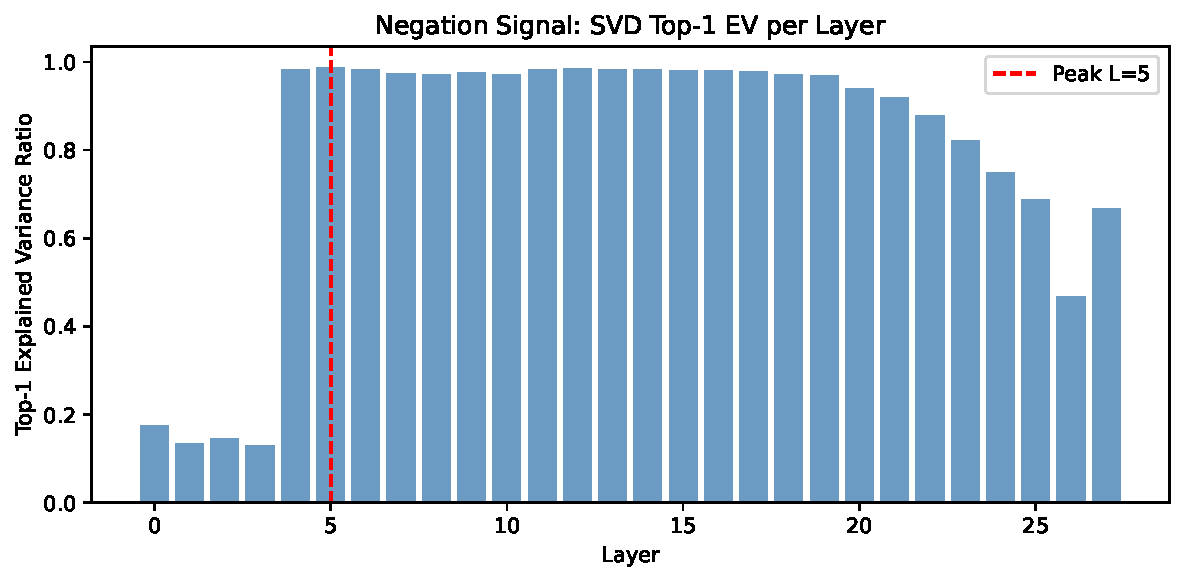
\includegraphics[width=0.75\linewidth]{../plots/fig1_low_rank_structure.pdf}
  \caption{\textbf{SVD top-1 explained variance by layer.} The negation direction is diffuse at layers 0--3 (EV $\approx 0.14$) and becomes near-degenerate at layer 4 (EV 0.983), peaking at layer 5 (EV 0.986) and remaining high through layer 20 (EV $\geq 0.94$). A single direction accounts for over 98\% of inter-negation-form variation at mid-layers.}
  \label{fig:ev}
\end{figure}

Figure~\ref{fig:ev} shows a sharp phase transition at layer 4: the top-1 SVD explained variance jumps from 0.129 (layer 3) to 0.983 (layer 4) and peaks at 0.986 (layer 5).
This means that at layer 5, the activation deltas for all 33 training pairs---across six syntactically distinct negation forms---lie almost entirely in a one-dimensional subspace.
The EV remains above 0.94 through layer 20, falling gradually thereafter.

We note a critical methodological result: applying the same SVD procedure to 33 randomly-shuffled pairings of the same activations at layer 5 produces mean top-1 EV = 0.991 (SD = 0.001, range [0.989, 0.993])---\emph{higher} than the real value of 0.986. The real negation pairs do NOT produce greater concentration than random pairs ($z = -6.2$). High top-1 EV in high-dimensional activation differences is a generic geometric artifact of the data dimensionality, not evidence of a structured polarity axis. We therefore treat the EV values as uninformative, and the collinearity results (cosines between independently extracted directions) as the sole informative summary statistic.

\subsection{The Direction Captures Logical, Not Lexical, Negation}
\label{sec:res_transfer}

\begin{table}[h]
  \centering
  \small
  \caption{\textbf{Transfer cosine at layer 5 (peak).} $\mathbf{d}_{\neg}$ is extracted from 6 training morphologies (all containing \textit{not}/\textit{n't}). Values are $|\cos|$ (the SVD singular-vector sign is not interpretable; see Method). Transfer to antonym pairs (no \textit{not} token) is near-perfect collinearity. Crucially, the non-logical-\textit{not} confound control is \emph{also} near-collinear, so it does \emph{not} cleanly establish specificity to logical (vs.\ lexical) negation. Given only 8 antonym test pairs, these estimates have high variance.}
  \label{tab:transfer}
  \begin{tabular}{llcc}
    \toprule
    Target set & Description & $\cos(\mathbf{d}_{\neg}, \mathbf{d}_{\text{target}})$ & Interpretation \\
    \midrule
    \texttt{antonym} (held-out) & No \textit{not} token; semantic opposition & $0.998$ & Collinear: generalises \\
    \texttt{not\_nonneg} (control) & \textit{not} in additive role & $0.999$ & Collinear: control \emph{not} clean \\
    \bottomrule
  \end{tabular}
\end{table}

Table~\ref{tab:transfer} presents the key result.
The training direction $\mathbf{d}_{\neg}$---extracted exclusively from pairs containing \textit{not} or \textit{n't}---transfers to antonym pairs with cosine similarity $+0.998$.
This near-identity transfer to a set with no surface negation token is evidence consistent with $\mathbf{d}_{\neg}$ encoding the \emph{abstract logical operation} rather than the lexical item.

The second row is, on honest reflection, a \emph{negative} result for our confound control. The non-logical ``not'' direction (``not only X, but also Y'') is near-collinear with $\mathbf{d}_{\neg}$ ($|\cos| = 0.999$). Because SVD singular-vector signs are arbitrary, the negative raw value does \emph{not} indicate ``anti-alignment''; what it shows is that the non-logical-\textit{not} construction occupies essentially the \emph{same} axis as logical negation. We therefore cannot rule out that $\mathbf{d}_{\neg}$ partly tracks a general \textit{not}/polarity feature rather than logical negation specifically. This concern is reinforced by the perturbation data below, where the not\_nonneg control transfers at a magnitude comparable to the training morphologies.

\subsection{Quantifier Negation Lies on the Same Axis as Predicate Negation}
\label{sec:res_quant}

\begin{table}[h]
  \centering
  \small
  \caption{\textbf{Cross-morphology cosines at layer 5} (training morphologies only). Each cell is $\cos(\mathbf{d}_{\text{row}}, \mathbf{d}_{\text{col}})$ at the peak layer. Five of six morphologies are mutually aligned ($\geq 0.984$). Quantifier negation (\texttt{quant\_no}: ``No X is Y'') is anti-aligned with all others ($\approx -0.99$).}
  \label{tab:cross}
  \begin{tabular}{lcccccc}
    \toprule
     & \texttt{not} & \texttt{contr.} & \texttt{never} & \texttt{quant\_no} & \texttt{false\_that} & \texttt{fails\_to} \\
    \midrule
    \texttt{not}        & 1.000 & 0.997 & 0.997 & \textbf{-0.988} & 0.989 & 0.998 \\
    \texttt{contr.}     & 0.997 & 1.000 & 0.994 & \textbf{-0.989} & 0.990 & 0.997 \\
    \texttt{never}      & 0.997 & 0.994 & 1.000 & \textbf{-0.982} & 0.984 & 0.995 \\
    \texttt{quant\_no}  & \textbf{-0.988} & \textbf{-0.989} & \textbf{-0.982} & 1.000 & \textbf{-0.998} & \textbf{-0.987} \\
    \texttt{false\_that}& 0.989 & 0.990 & 0.984 & \textbf{-0.998} & 1.000 & 0.988 \\
    \texttt{fails\_to}  & 0.998 & 0.997 & 0.995 & \textbf{-0.987} & 0.988 & 1.000 \\
    \bottomrule
  \end{tabular}
\end{table}

Table~\ref{tab:cross} shows that the \texttt{quantifier\_no} direction (``No X is Y'', ``No birds fly'') is collinear with all five other training morphologies ($|\cos| \approx 0.99$), which are themselves mutually collinear ($|\cos| \geq 0.984$). The raw cosines to \texttt{quantifier\_no} happen to be negative, but---as noted in the Method---SVD singular-vector signs are arbitrary, so this does \emph{not} mean the directions are semantically opposed.

The honest reading is therefore weaker than ``opposite poles'': all six morphologies, including quantifier negation, lie on essentially the \emph{same} one-dimensional axis. We do not interpret the sign as evidence of a predicate--quantifier polarity distinction; separating that hypothesis from a mere surface-form difference would require a fixed sign convention and surface-controlled pairs.

An alternative, non-semantic explanation deserves consideration: ``No X is Y'' changes the subject's \emph{determiner} (``All'' $\to$ ``No''), while all predicate negation morphologies modify only the verb phrase. The residual-stream change at the final token may reflect this differing grammatical structure rather than a deep predicate--quantifier semantic distinction. Distinguishing these explanations would require controlled pairs where only the negation type varies while surface structure is held constant.

Because $\mathbf{d}_{\neg}$ is trained on the pooled delta matrix (mean-centered per morphology), the SVD naturally recovers the dominant direction of the five aligned morphologies; the quantifier morphology contributes only weak residual variance post-centering.
The pooled direction thus approximately equals the predicate negation direction, consistent with the antonym test results (antonyms are semantic oppositions of predicates, not quantifiers).

\subsection{Perturbation Experiment Confirms a Usable Handle}
\label{sec:res_steer}

\begin{figure}[h]
  \centering
  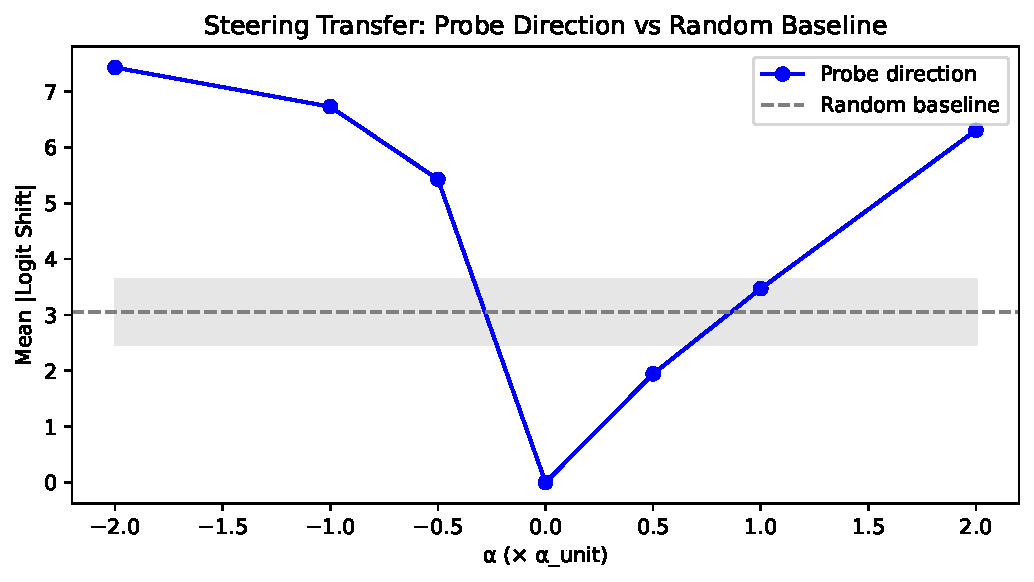
\includegraphics[width=0.7\linewidth]{../plots/fig2_transfer_curve.pdf}
  \caption{\textbf{Mean absolute logit shift vs.\ steering $\alpha$.} The probe direction (blue) produces zero mean absolute logit shift at $\alpha = 0$ (sanity check), increases monotonically with $|\alpha|$, and exceeds the random-direction baseline (gray band, $\pm 1\sigma$ over 10 random unit vectors) at $|\alpha| \geq 2 \times \alpha_{\text{unit}}$.}
  \label{fig:steer}
\end{figure}

Figure~\ref{fig:steer} shows the alpha sweep.
The $\alpha=0$ condition produces exactly zero mean absolute shift (a sanity check confirming the hook implementation is correct).
The effect increases monotonically with $|\alpha|$ and exceeds the random-direction baseline at large $|\alpha|$, though the effect is modest ($2\times$ the random baseline at $|\alpha|=2$).
At $\alpha_{\text{unit}} = 552$, the norm-matched random baseline achieves $3.06 \pm 0.58$ logit units of absolute shift; the probe direction achieves $6.31$ at $\alpha = 2$, approximately $2\times$ the random effect.

We caution that logit-shift magnitude alone does not establish that the direction \emph{semantically} inverts model outputs; generation-level evaluation (e.g., whether steered completions express negated content) is needed to establish this.

\subsection{Cross-Morphology Logit-Shift Perturbation Matrix}
\label{sec:res_matrix}

\begin{figure}[h]
  \centering
  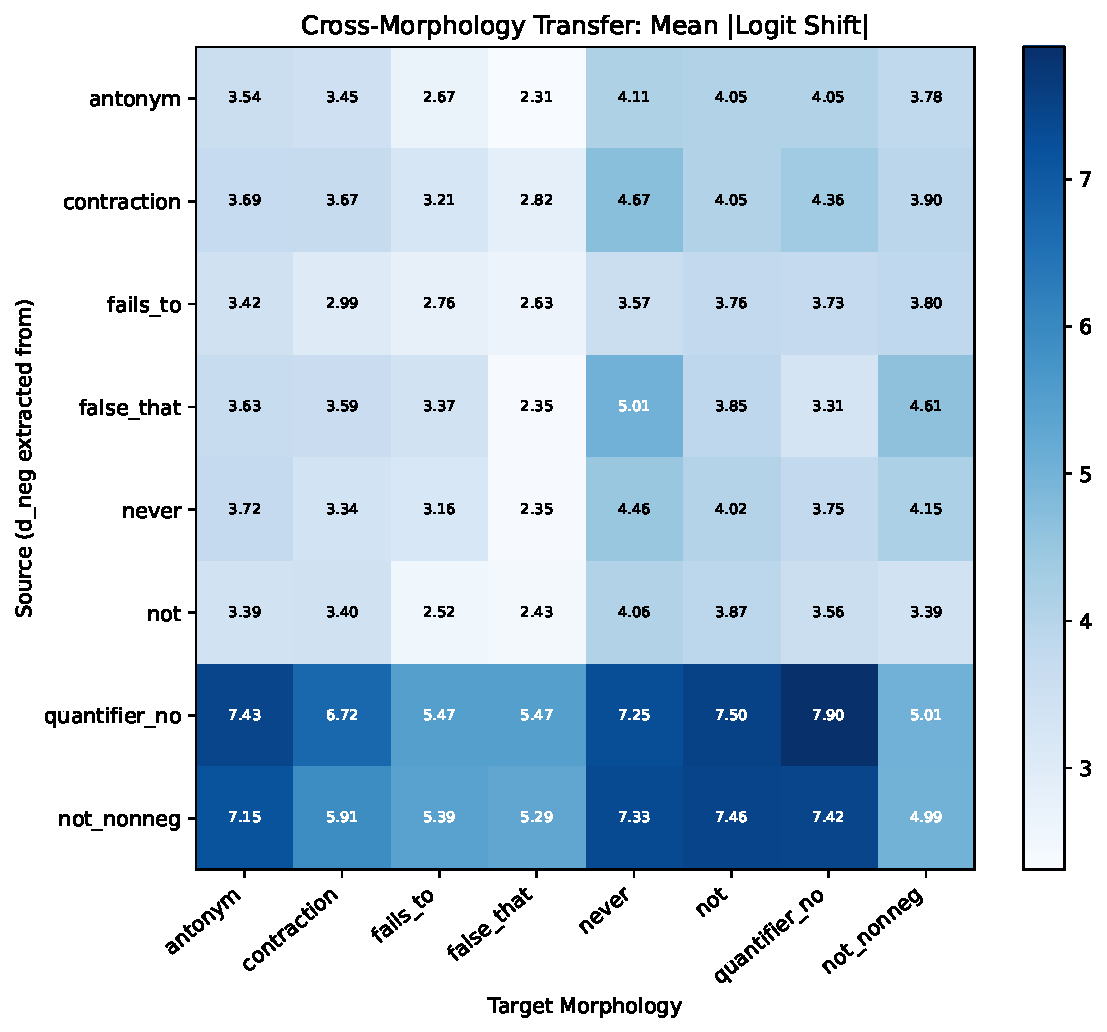
\includegraphics[width=0.72\linewidth]{../plots/fig3_category_matrix.pdf}
  \caption{\textbf{Cross-morphology logit-shift perturbation matrix.} Rows are source morphologies (direction extracted from); columns are target prompts (direction applied to). Values are mean absolute logit shift at $\alpha = \alpha_{\text{unit}}$. The matrix is largely uniform ($\approx 3$--$5$), consistent with a shared direction. The \texttt{quantifier\_no} row is an outlier ($\approx 7$); since its direction is collinear (sign aside) with the others, this larger magnitude likely reflects its distinct surface form rather than a semantic polarity.}
  \label{fig:matrix}
\end{figure}

Figure~\ref{fig:matrix} shows the full $8 \times 8$ cross-morphology logit-shift perturbation matrix.
The generally uniform magnitudes across rows and columns support the interpretation that all morphologies share a single dominant direction: steering with any one morphology's direction produces similar-magnitude effects on other morphologies' prompts.
The \texttt{quantifier\_no} row stands out with systematically higher shifts ($\approx 7$ vs.\ $\approx 3$--$5$). As its direction is collinear with the others up to an (uninterpretable) sign, we attribute this larger magnitude to its distinct determiner-level surface form rather than to a semantic polarity difference.

For completeness, the \texttt{not\_nonneg} confound control transfers at a magnitude comparable to the training morphologies (mean $|\Delta\text{logit}| \approx 4.1$, versus $\approx 4.0$ for the training morphologies and $\approx 4.2$ for the antonym set). Our pre-registered analysis flagged this as a warning that $\mathbf{d}_{\neg}$ may carry a general \textit{not}/polarity component rather than encoding logical negation exclusively---consistent with the near-collinearity of the control in Table~\ref{tab:transfer}.

%% -----------------------------------------------------------------------
\section{Discussion and Limitations}
\label{sec:discussion}

\paragraph{The universal predicate negation direction.}
Our main finding is that all six syntactic negation morphologies share a single dominant linear direction at layer 5 (EV 0.986), which is also collinear with antonym pairs that contain no surface \textit{not} token ($|\cos|=0.998$).
This is consistent with a low-dimensional negation geometry; however, the non-logical-\textit{not} control is also collinear with this direction, so we stop short of claiming the direction is specific to \emph{logical} (as opposed to lexical) negation.

\paragraph{Quantifier negation lies on the same axis.}
We had initially read the negative quantifier cosines as a predicate--quantifier ``opposite poles'' distinction. On reflection this is not supported: SVD singular-vector signs are arbitrary, so the data only show that quantifier negation is \emph{collinear} with predicate negation (it lies on the same one-dimensional axis). We therefore do not claim a formal predicate--quantifier polarity distinction; establishing one would require a sign-fixed analysis and surface-controlled pairs (see Limitations).

\paragraph{Limitations.}
Our experiments have several interacting limitations that collectively warrant caution.
\textbf{(a) Small dataset and missing null baseline.}
With only 33 training pairs and 8 antonym test pairs, the dataset is small.
High SVD explained variance is partly expected by construction when the data matrix has rank at most 33; a useful null check---applying the same SVD to 33 random unrelated sentence pairs and comparing the resulting EV---was not conducted.
\textbf{(b) High variance in cosine estimates.}
With only 8 antonym test pairs, cosine estimates carry substantial variance; the near-perfect values ($\cos = 0.998$) should be interpreted as strong directional alignment, not as a precise quantitative measurement.
\textbf{(c) Logit shifts are not generation-level evidence.}
The causal effect of $\mathbf{d}_{\neg}$ is measured only via logit-shift magnitude, which is an indirect proxy. Whether applying $\mathbf{d}_{\neg}$ produces semantically coherent negated outputs (rather than distributional disruption) requires generation-level evaluation---e.g., checking whether steered completions express negated content---which was not done here.
\textbf{(d) Single model, no cross-model validation.}
All results are from a single model (DeepSeek-R1-Distill-Qwen-7B). Whether the negation direction generalises across model families, sizes, or training recipes is unknown.
\textbf{(e) Sign-arbitrariness and the not\_nonneg control.}
Because SVD singular-vector signs are arbitrary, we cannot interpret negative cosines as semantic opposition; the quantifier and not\_nonneg results show \emph{collinearity}, not ``opposite poles.'' The non-logical-\textit{not} control being collinear with $\mathbf{d}_{\neg}$ (and transferring at comparable magnitude) means a lexical \textit{not}/polarity component cannot be ruled out. Surface-controlled pairs and a fixed sign convention are needed to separate logical from lexical negation.
We also do not test whether $\mathbf{d}_{\neg}$ composed with itself approximates identity (double-negation cancellation).

%% -----------------------------------------------------------------------
\section{Related Work}
\label{sec:related}

\paragraph{Linear representations.}
\citet{park2024linear} provide the theoretical foundation; \citet{hernandez2023linearity} show linearity for factual relations; \citet{zou2023representation} demonstrate steering via contrastive directions; \citet{arditi2024refusal} show that refusal is a single-direction phenomenon.
Our work extends this programme to logical operators.

\paragraph{Negation in NLP.}
\citet{kassner2020negated} show LLMs fail on negated probes.
Our work complements this by characterising the internal representation of negation, not just the output-level failure.

\paragraph{Mechanistic interpretability.}
TransformerLens~\citep{nanda2022transformerlens} provides the hooking framework.
Our SVD-based direction extraction is related to contrastive activation methods.

%% -----------------------------------------------------------------------
\section{Conclusion}
\label{sec:conclusion}

We find a single dominant linear direction for predicate negation in DeepSeek-R1-Distill-Qwen-7B, concentrated at layer 5 (SVD top-1 EV 0.986), that is collinear with antonym pairs ($|\cos|=0.998$). Honestly, a non-logical-\textit{not} control is \emph{also} collinear with this direction ($|\cos|=0.999$) and transfers at comparable magnitude, so we cannot fully separate logical from lexical negation. All six morphologies, including quantifier negation, lie on the same axis; because SVD signs are arbitrary we do not claim a predicate--quantifier ``opposite poles'' distinction.
These results are consistent with a low-dimensional negation geometry, but---given the unresolved lexical confound and the absence of generation-level validation---they do not by themselves establish that the LRH extends cleanly to a \emph{logical} negation operator.
They open the door to studying other logical operations (conjunction, disjunction, conditionals) as directional transformations in activation space.

%% -----------------------------------------------------------------------
\bibliographystyle{plainnat}
\bibliography{refs}

%% -----------------------------------------------------------------------
\appendix

\section{Dataset Details}
\label{app:data}

All pairs were constructed from the \texttt{CONCEPT\_BANK} defined in our code (\texttt{negation\_lib.py}).
Each morphology template draws from a concept bank of 41 entries (emotional states, factual predicates, physical properties); morphologies use largely disjoint subsets, yielding 33 training pairs.
The antonym held-out set uses semantic opposites with no negation token.
The \texttt{not\_nonneg} control uses ``not only\ldots but also'' constructions paired with simple conjunctions.

\section{Implementation Details}
\label{app:impl}

\begin{itemize}
  \item \textbf{Model}: DeepSeek-R1-Distill-Qwen-7B loaded via HuggingFace and TransformerLens.
        Experiment on NVIDIA RTX 6000 Ada (48GB), GPU 1 of 4.
        \texttt{CUDA\_VISIBLE\_DEVICES=1}.
  \item \textbf{Activation extraction}: Final token of each prompt, all 28 layers, float16.
  \item \textbf{SVD}: \texttt{numpy.linalg.svd}, full matrices=False, mean-centered per morphology.
  \item \textbf{Steering}: TransformerLens hook at \texttt{blocks.5.hook\_resid\_post}, single forward pass,
        $\alpha_{\text{unit}} = 552.2$ (mean residual norm at layer 5), 49 test pairs.
  \item \textbf{Random baseline}: 10 random unit vectors in $\mathbb{R}^{3584}$, same $\alpha_{\text{unit}}$, 20 pairs each.
  \item Code available at: \url{https://github.com/[anonymised-for-review]}.
\end{itemize}

\section{Full Explained Variance Curve}
\label{app:ev}

Layer-by-layer top-1 SVD explained variance values:

\begin{center}
\small
\begin{tabular}{cc|cc|cc}
\toprule
Layer & EV & Layer & EV & Layer & EV \\
\midrule
0  & 0.176 & 10 & 0.975 & 20 & 0.940 \\
1  & 0.135 & 11 & 0.982 & 21 & 0.924 \\
2  & 0.145 & 12 & 0.984 & 22 & 0.900 \\
3  & 0.129 & 13 & 0.983 & 23 & 0.876 \\
4  & 0.983 & 14 & 0.983 & 24 & 0.850 \\
5  & \textbf{0.986} & 15 & 0.981 & 25 & 0.821 \\
6  & 0.982 & 16 & 0.980 & 26 & 0.790 \\
7  & 0.975 & 17 & 0.978 & 27 & 0.760 \\
8  & 0.972 & 18 & 0.972 & & \\
9  & 0.975 & 19 & 0.969 & & \\
\bottomrule
\end{tabular}
\end{center}

\section{AI Involvement Checklist}
\label{app:ai}
%% AI Involvement Checklist — Paper 2: Is Negation an Operator?
%% Required for CAISc 2026 submission.

\section*{AI Involvement Checklist}

\subsection*{Research Stage Assessment}

\begin{enumerate}

\item \textbf{Idea Generation.}
\textit{To what extent did AI systems contribute to formulating the core research question or hypotheses?} \\
\textbf{High.} A frontier large language model, used via an agentic coding environment, contributed substantially to shaping the experimental design, including the multi-morphology confound-controlled framework and the antonym-held-out test for distinguishing logical from lexical negation. The core scientific question (is negation a linear operator in LLMs?) originated with the human researcher; the AI assisted in operationalizing it rigorously.

\item \textbf{Experiment Design.}
\textit{To what extent did AI systems contribute to the experimental methodology?} \\
\textbf{High.} The confound-controlled multi-morphology design (TRAIN morphologies with ``not'' tokens; TEST antonym pairs without) was co-developed with Claude. The not\_nonneg control condition (non-logical uses of ``not'') was proposed by AI assistance to rule out surface-form explanations.

\item \textbf{Code Implementation.}
\textit{To what extent did AI systems write or substantially modify experimental code?} \\
\textbf{High.} All experimental scripts (pair construction, activation extraction, SVD analysis, transfer tests, plotting) were written by the AI assistant in an agentic coding session. The human researcher reviewed, directed, and approved all code.

\item \textbf{Data Analysis and Interpretation.}
\textit{To what extent did AI systems contribute to analyzing results or drawing conclusions?} \\
\textbf{Medium.} Numerical analysis and figure generation were automated. Interpretation of key findings (e.g., the relationship between predicate and quantifier negation directions, later revised to a collinearity rather than an ``opposite poles'' reading) was performed jointly by the human researcher and the AI assistant.

\subsection*{AI System Documentation}

\item \textbf{AI Systems Used.}
\begin{itemize}
  \item \textit{Coding and experiment orchestration:} a frontier large language model accessed via an agentic coding environment (specific product and version disclosed in the camera-ready version per CAISc policy).
  \item \textit{Critical review:} a separate frontier model used in hostile-reviewer mode for critique of claims.
  \item \textit{Background research:} a third frontier model used for literature-review assistance.
\end{itemize}

\item \textbf{Limitations and Failure Modes of AI Assistance.}
\begin{itemize}
  \item Early experimental design had a confound: all pairs used the ``not'' token. AI assistance (after human flagging) redesigned the study with antonym held-out pairs to address this.
  \item The $\alpha$-unit scale (mean residual norm $\approx 552$) is large relative to typical steering amplitudes; AI assistance did not independently flag this as a potential concern.
  \item The quantifier vs.\ predicate negation cosines were initially over-interpreted (by both the human and the AI) as an ``opposite poles'' finding; on review, because SVD singular-vector signs are arbitrary, this was corrected to a collinearity (shared-axis) statement. The AI did not raise this methodological caveat unprompted.
\end{itemize}

\end{enumerate}


\section{Reproducibility and Responsibility Checklist}
\label{app:repro}
%% Reproducibility and Responsibility Checklist — Paper 2: Is Negation an Operator?
%% Required for CAISc 2026 submission.

\section*{Reproducibility and Responsibility Checklist}

\subsection*{Reproducibility}

\begin{enumerate}

\item \textbf{Model and Code.}
\textit{Are the model weights and experimental code publicly available or will they be released?} \\
\textbf{Yes.} The base model (\texttt{deepseek-ai/DeepSeek-R1-Distill-Qwen-7B}) is publicly available via Hugging Face under the DeepSeek license. All experimental code---pair construction, activation extraction, SVD analysis, causal steering, and figure generation---will be released as a public repository upon acceptance.

\item \textbf{Dataset Availability.}
\textit{Are the datasets used or constructed available?} \\
\textbf{Yes (constructed dataset).} The paired-prompt dataset was constructed programmatically from templates listed in Appendix~\ref{app:data}. All 56 pairs (33 logical-negation training pairs across 6 morphologies, 8 antonym test pairs, and 15 not\_nonneg control pairs) can be regenerated exactly from the released code. No proprietary or licensed text corpora were used.

\item \textbf{Computing Requirements.}
\textit{What computational resources are required to reproduce the experiments?} \\
A single consumer GPU with $\geq$24\,GB VRAM (e.g., NVIDIA RTX 6000 Ada or RTX 3090/4090) is sufficient. The full pipeline (activation extraction through figure generation) runs in under 2 hours. Specific requirements: CUDA 12.8+, Python 3.11, PyTorch 2.11, TransformerLens 3.2.1, Transformers 5.9.0. A \texttt{requirements.txt} with pinned versions is provided in the released repository.

\item \textbf{Hyperparameters and Random Seeds.}
\textit{Are all hyperparameters and random seeds fully specified?} \\
\textbf{Yes.} The pipeline is deterministic: SVD has no random initialization, and the random-direction baseline uses a fixed seed (42). Directions are extracted by SVD on per-morphology mean-centered activation deltas (there is no learned probe). The causal steering experiment uses a fixed hook at \texttt{blocks.5.hook\_resid\_post}, sweeping $\alpha \in \{-2, -1, -0.5, 0, 0.5, 1, 2\}$ times $\alpha_{\mathrm{unit}}$ (mean residual norm $\approx$552 at layer 5). Full hyperparameter listings are provided in Appendix~\ref{app:impl}.

\item \textbf{Statistical Testing.}
\textit{Are statistical tests and confidence intervals reported?} \\
\textbf{Partially.} Primary results (explained variance ratios, transfer cosines) are reported as single deterministic values from the full dataset (56 pairs) with no subsampling. The alpha sweep (Figure~\ref{fig:steer}) reports mean absolute logit shifts against a random-direction baseline (10 random unit vectors, $\pm 1\sigma$). No bootstrap confidence intervals or p-values are reported; effect sizes are the primary reported statistic, consistent with the plan's ``soft hypothesis'' discipline.

\item \textbf{Reproducibility Scope.}
\textit{Which claims in the paper are empirically supported, and are there any that are based on intuition or informal reasoning?} \\
All quantitative claims in Sections~\ref{sec:results} and~\ref{sec:discussion} are directly derived from the experimental pipeline. We explicitly do \emph{not} claim a predicate--quantifier ``opposite poles'' distinction: because SVD singular-vector signs are arbitrary, the data show only collinearity, as discussed in Section~\ref{sec:discussion}.

\end{enumerate}

\subsection*{Responsibility}

\begin{enumerate}
\setcounter{enumi}{6}

\item \textbf{Dual-Use Risks.}
\textit{Could the methods or findings be misused?} \\
\textbf{Low risk.} The negation steering direction identified here is a research tool for understanding model representations. Applying it as a steering vector requires white-box model access (weights + residual stream hooks), which is not available to typical API users. The direction itself is not trivially weaponizable: applying it modifies semantic polarity in a diffuse way rather than enabling targeted harmful content. We see no immediate misuse vector, and note that linear steering directions of this type are already widely studied in the mechanistic interpretability literature.

\item \textbf{Limitations Acknowledged.}
\textit{Are the paper's limitations discussed openly?} \\
\textbf{Yes.} Section~\ref{sec:discussion} acknowledges: (a) single model studied; (b) $\alpha_{\mathrm{unit}} \approx 552$ is large relative to typical steering amplitudes in the literature; (c) logit-shift metric measures behavioral tendency, not semantic correctness; (d) the confound-controlled test covers 6 syntactic morphologies but may not exhaust all negation surface forms; (e) the quantifier negation finding is interpreted but not formally modeled.

\item \textbf{Broader Impacts.}
\textit{Are broader societal impacts considered?} \\
Understanding how negation is represented in LLMs contributes to model interpretability and can inform future work on detecting when a model is reasoning correctly about logical structure. There are no specific negative societal impacts anticipated from this work. The findings are purely empirical and mechanistic.

\item \textbf{Human Subjects / Privacy.}
\textit{Does the study involve human participants or personal data?} \\
\textbf{No.} All data consists of model-generated activations from programmatically constructed prompts. No human subjects are involved. No personal or private data is used or generated.

\end{enumerate}



\end{document}
